\documentclass[10pt,aspectratio=169]{beamer}

\usetheme{default}
\useinnertheme{rounded}

\usepackage[utf8]{inputenc}
\usepackage[T1]{fontenc}
\usepackage[french]{babel}
\usepackage{lmodern}
\usepackage{graphicx}
\usepackage{booktabs}
\usepackage{array}
\usepackage{colortbl}
\usepackage{pifont}
\usepackage{tikz}
\usetikzlibrary{arrows.meta,positioning,shapes.geometric,calc,shadows}
\usepackage{pgfplots}
\pgfplotsset{compat=1.18}

\graphicspath{{assets/}{../memoire-doc/}}

\definecolor{NanterreBlue}{RGB}{55,52,180}
\definecolor{ProfBlack}{RGB}{0,0,0}
\definecolor{NavMuted}{RGB}{150,150,160}
\definecolor{AgigaGreen}{RGB}{40,139,98}
\definecolor{SoftBlue}{RGB}{232,232,248}
\definecolor{SoftGreen}{RGB}{228,243,235}
\definecolor{SoftOrange}{RGB}{250,235,214}
\definecolor{SoftRed}{RGB}{247,226,226}
\definecolor{TextGray}{RGB}{60,65,72}

\setbeamercolor{structure}{fg=NanterreBlue}
\setbeamercolor{frametitle}{fg=white,bg=NanterreBlue}
\setbeamercolor{title}{fg=NanterreBlue}
\setbeamercolor{block title}{fg=white,bg=NanterreBlue}
\setbeamercolor{block body}{fg=black,bg=SoftBlue}
\setbeamercolor{alerted text}{fg=AgigaGreen}
\setbeamercolor{section in head/foot}{fg=white,bg=ProfBlack}
\setbeamercolor{subsection in head/foot}{fg=white,bg=NanterreBlue}
\setbeamercolor{author in head/foot}{fg=white,bg=ProfBlack}
\setbeamercolor{title in head/foot}{fg=white,bg=NanterreBlue}
\setbeamerfont{headline title}{series=\bfseries,size=\normalsize}
\setbeamerfont{footline text}{series=\bfseries,size=\scriptsize}
\setbeamertemplate{frametitle}{}
\setbeamertemplate{blocks}[rounded][shadow=true]
\setbeamertemplate{navigation symbols}{%
  \insertslidenavigationsymbol%
  \insertframenavigationsymbol%
  \insertsubsectionnavigationsymbol%
  \insertsectionnavigationsymbol%
  \insertdocnavigationsymbol%
  \insertbackfindforwardnavigationsymbol%
}
\setbeamertemplate{itemize item}{\raise0.18ex\hbox{\scriptsize$\blacktriangleright$}}
\setbeamertemplate{itemize subitem}{\raise0.18ex\hbox{\tiny$\bullet$}}
\setbeamercolor{navigation symbols}{fg=NanterreBlue!30,bg=white}
\setbeamercolor{navigation symbols dimmed}{fg=NanterreBlue!15,bg=white}
\makeatletter
\def\beamer@shortframetitle{}
\makeatother

\setbeamertemplate{headline}{%
  \leavevmode%
  \hbox{%
    \begin{beamercolorbox}[wd=.50\paperwidth,ht=1.12cm,dp=.16cm,right,rightskip=.35cm]{section in head/foot}%
      \parbox[c][.92cm][c]{.46\paperwidth}{\raggedleft\usebeamerfont{headline title}\insertsection}
    \end{beamercolorbox}%
    \begin{beamercolorbox}[wd=.50\paperwidth,ht=1.12cm,dp=.16cm,left,leftskip=.35cm]{subsection in head/foot}%
      \parbox[c][.92cm][c]{.46\paperwidth}{\raggedright\usebeamerfont{headline title}\insertshortframetitle}
    \end{beamercolorbox}%
  }%
  \vskip0pt%
  \hbox{\color{black!25}\rule{\paperwidth}{0.7pt}}%
}

\setbeamertemplate{footline}{%
  \leavevmode%
  \hbox{%
    \begin{beamercolorbox}[wd=.50\paperwidth,ht=.33cm,dp=.08cm,left,leftskip=.35cm]{author in head/foot}%
      \usebeamerfont{footline text} Seyed Amineddin Miri
    \end{beamercolorbox}%
    \begin{beamercolorbox}[wd=.50\paperwidth,ht=.33cm,dp=.08cm,left,leftskip=.35cm,rightskip=.25cm]{title in head/foot}%
      \usebeamerfont{footline text} A Systematic Mapping Study of Learned Indexes \hfill \insertframenumber/\inserttotalframenumber
    \end{beamercolorbox}%
  }%
}

\newcommand{\smallcaps}[1]{\textsc{\MakeLowercase{#1}}}
\newcommand{\keypoint}[1]{%
  \begin{center}
  \begin{tikzpicture}
    \node[draw=NanterreBlue, fill=NanterreBlue, rounded corners=3pt, drop shadow={shadow xshift=4pt, shadow yshift=-4pt, opacity=.35}, inner xsep=12pt, inner ysep=11pt, text width=0.86\linewidth, align=center, text=white] {\large #1};
  \end{tikzpicture}
  \end{center}
}

\title[A Systematic Mapping Study of Learned Indexes]{A Systematic Mapping Study of Learned Indexes in Database Systems}
\subtitle{Soutenance M1 MIAGE — édition publique (contenu employeur masqué)}
\author[Seyed Amineddin Miri]{Seyed Amineddin Miri}
\institute[Université Paris Nanterre]{%
  Université Paris Nanterre \\
  Entreprise : Agiga \\
  Fonction : Full Stack Developer
}
\date{Juin 2026}

\begin{document}

\begin{frame}[plain]
  \vspace{0.5cm}
  \begin{center}
    {\Large\bfseries\color{NanterreBlue} A Systematic Mapping Study of Learned Indexes\\in Database Systems}

    \vspace{0.35cm}
    {\large Soutenance M1 MIAGE — édition publique }

    \vspace{0.55cm}
    {\large Seyed Amineddin Miri}

    \vspace{0.25cm}
    {\small Université Paris Nanterre\\
    Entreprise : Agiga\\
    Fonction : Full Stack Developer}
  \end{center}

  \vspace{0.45cm}
  \begin{center}
    
\includegraphics[height=0.65cm]{logo_Paris_Nanterre_couleur_RVB.png}
    \hspace{1.2cm}
    
\includegraphics[height=0.65cm]{logo_entreprise.png}
  \end{center}
  \vspace{0.45cm}
  \begin{columns}[T,onlytextwidth]
    \begin{column}{0.33\textwidth}
      \centering\scriptsize
      Tuteur enseignant : Pascal Poizat
    \end{column}
    \begin{column}{0.34\textwidth}
      \centering\scriptsize
      Responsable du master : François Delbot
    \end{column}
    \begin{column}{0.33\textwidth}
      \centering\scriptsize
      Maître d'apprentissage : Nicolas Loriot
    \end{column}
  \end{columns}
\end{frame}

\section{Activité en entreprise}

% Employer-related content is omitted from both the source and the public PDF.
\newcommand{\employerredaction}{%
  \vfill
  \begin{center}
    {\Large\bfseries\color{NanterreBlue} CONTENU MASQUÉ / REDACTED}

    \vspace{0.6cm}
    \begin{minipage}{0.78\textwidth}
      \centering
      Le contenu de cette diapositive concerne mon employeur.\\[0.2cm]
      Il a été retiré de la version publique pour préserver la confidentialité des informations de l'entreprise.
    \end{minipage}
  \end{center}
  \vfill
}

\begin{frame}{Contenu employeur masqué}
  \employerredaction
\end{frame}

\begin{frame}{Contenu employeur masqué}
  \employerredaction
\end{frame}

\begin{frame}{Contenu employeur masqué}
  \employerredaction
\end{frame}

\section{Contexte technique}

\begin{frame}{Qu'est-ce qu'un learned index ?}
  \begin{columns}[T,onlytextwidth]
    \begin{column}{0.48\textwidth}
      \begin{itemize}
        \item Un index évite de scanner toute une table. Les structures classiques (B+-trees, hash, radix) sont robustes, mais leur efficacité dépend du contexte.
        \item Idée : un index peut être vu comme une fonction.
        \item Pour des données triées, on apprend la relation :
      \end{itemize}
      \begin{center}
      \large\texttt{clé} $\rightarrow$ position approximative
      \end{center}
      \begin{itemize}
        \item Le modèle prédit une position.
        \item Une étape de correction peut être utilisée pour garantir le résultat exact.
      \end{itemize}
    \end{column}
    \begin{column}{0.50\textwidth}
      \centering
      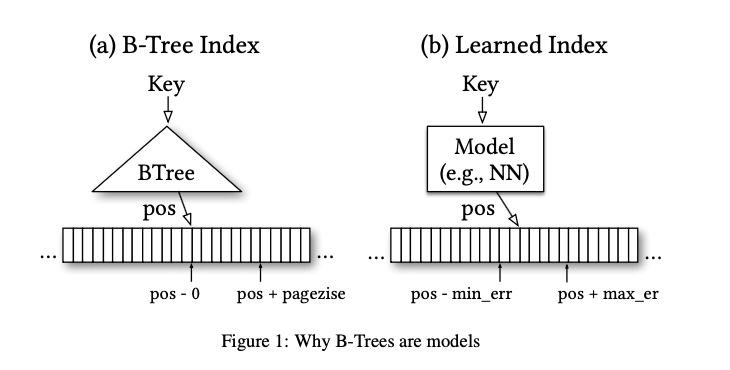
\includegraphics[height=2.75cm]{fig-btree-vs-learned.png}\\[0.15cm]
      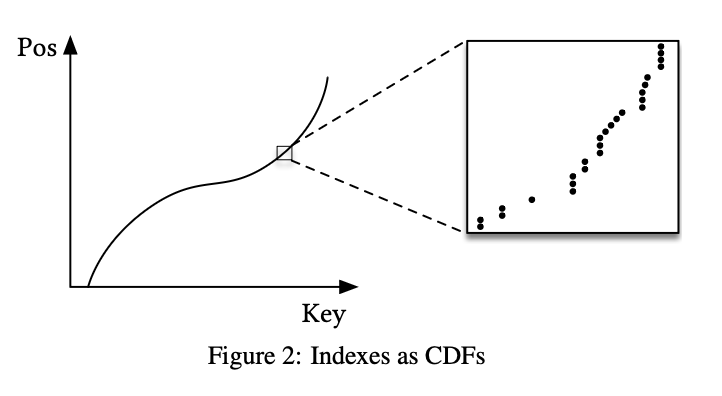
\includegraphics[height=2.75cm]{fig-cdf.png}\\[0.1cm]
      {\tiny Figures : Kraska et al., \emph{The Case for Learned Index Structures} (2018).}
    \end{column}
  \end{columns}
\end{frame}

\begin{frame}{Index classique vs learned index}
  \begin{columns}[T,onlytextwidth]
    \begin{column}{0.48\textwidth}
      \begin{block}{Index classique}
        \begin{itemize}
          \item Structure générale et robuste.
          \item Moins sensible à la distribution des données.
          \item Très bon comportement dans beaucoup de contextes.
        \end{itemize}
      \end{block}
    \end{column}
    \begin{column}{0.48\textwidth}
      \begin{block}{Learned index}
        \begin{itemize}
          \item Exploite la distribution des données.
          \item Peut être plus compact ou plus rapide quand la distribution et le workload s'y prêtent.
          \item Peut nécessiter une étape de correction et du tuning.
        \end{itemize}
      \end{block}
    \end{column}
  \end{columns}

  \vspace{0.45cm}
  \keypoint{Les deux approches sont utiles : la vraie question n'est pas \emph{laquelle remplace l'autre}, mais \emph{dans quels contextes} le learned index devient intéressant.}
\end{frame}

\section{Méthodologie SMS}

\begin{frame}{Pourquoi une Systematic Mapping Study ?}
  \begin{itemize}
    \item Domaine récent (papier fondateur en 2018), déjà très hétérogène : les papiers ne comparent ni les mêmes structures, ni les mêmes métriques, ni les mêmes contextes.
  \end{itemize}

  \vspace{0.35cm}
  \begin{center}
  \small
  \renewcommand{\arraystretch}{1.45}
  \setlength{\tabcolsep}{6pt}
  \begin{tabular}{>{\raggedright\arraybackslash}p{2.1cm}>{\raggedright\arraybackslash}p{4.4cm}>{\raggedright\arraybackslash}p{4.4cm}}
    \toprule
     & \textbf{SLR} {\footnotesize(revue systématique)} & \textbf{SMS} {\footnotesize(cartographie)} \\
    \midrule
    Question & «~Quelle approche est la meilleure ?~» & «~Qu'a-t-on étudié, et que manque-t-il ?~» \\
    Suppose & des résultats agrégeables & accepte des études hétérogènes \\
    Produit & un verdict & une carte : familles couvertes + zones peu étudiées \\
    Adaptée à & un champ mûr & un champ jeune \\
    \bottomrule
  \end{tabular}
  \end{center}

  \vspace{0.3cm}
  \footnotesize
  Des surveys existent déjà, mais restent souvent très larges ; ce mémoire se distingue par des questions de recherche plus ciblées et un protocole explicite de sélection et de classification.
\end{frame}

\begin{frame}{Questions de recherche et corpus}
  \vspace{0.15cm}
  \begin{center}
    {\small\itshape\color{NanterreBlue} Le learned index remplace-t-il l'index classique, ou son gain est-il seulement conditionnel ?}
  \end{center}
  \vspace{0.2cm}
  \begin{columns}[T,onlytextwidth]
    \begin{column}{0.48\textwidth}
      \begin{block}{Questions de recherche}
        \footnotesize
        \begin{itemize}
          \item \textbf{RQ1} — Quels types d'études sur les learned indexes ont été publiés, et comment se répartissent-ils dans le temps et selon les lieux de publication ?
          \item \textbf{RQ2} — Quelles techniques de learned indexes et quels scénarios de workload sont traités dans la littérature ?
          \item \textbf{RQ3} — Comment les learned indexes sont-ils évalués, et quelles preuves a-t-on sur la performance, la robustesse et la reproductibilité ?
        \end{itemize}
      \end{block}
      \vspace{0.15cm}
    \end{column}
    \begin{column}{0.06\textwidth}\end{column}
    \begin{column}{0.44\textwidth}
      \begin{tikzpicture}[
        node distance=0.38cm,
        box/.style={draw=TextGray, rounded corners=2pt, align=center, text width=4.55cm, minimum height=0.55cm, font=\scriptsize},
        arrow/.style={-{Latex[length=1.8mm]}, thick, draw=TextGray}
      ]
        \node[box, fill=SoftBlue] (raw) {1 396 records collectés};
        \node[box, fill=SoftBlue, below=of raw] (unique) {931 records uniques};
        \node[box, fill=SoftOrange, below=of unique] (short) {90 papiers présélectionnés};
        \node[box, fill=SoftGreen, below=of short] (snow) {16 papiers retenus via seeds/snowballing};
        \node[box, fill=SoftGreen, below=of snow] (target) {+ 2 via recherche ciblée};
        \node[box, fill=AgigaGreen!18, draw=AgigaGreen, below=of target] (final) {\textbf{18 études primaires}};
        \draw[arrow] (raw) -- (unique);
        \draw[arrow] (unique) -- (short);
        \draw[arrow] (short) -- (snow);
        \draw[arrow] (snow) -- (target);
        \draw[arrow] (target) -- (final);
      \end{tikzpicture}
    \end{column}
  \end{columns}

  \vspace{0.2cm}
  {\footnotesize\centering Je terminerai par trois résultats concrets du corpus pour l'illustrer.\par}
\end{frame}

\section{Résultats}

\begin{frame}{RQ1 -- Un domaine qui s'est diversifié}
  \begin{columns}[T,onlytextwidth]
    \begin{column}{0.35\textwidth}
      \begin{itemize}
        \item 2018--2019 : idée fondatrice et premières structures.
        \item 2020--2022 : index dynamiques, benchmarks, analyses critiques.
        \item 2023--2026 : robustesse, disque, tuning, intégration dans PostgreSQL/LeanStore.
      \end{itemize}
      \vspace{0.2cm}
    \end{column}
    \begin{column}{0.63\textwidth}
      \centering
      {\scriptsize Distribution par année}\\[-0.1cm]
      \begin{tikzpicture}
        \begin{axis}[
          width=7.75cm,
          height=2.75cm,
          ybar,
          bar width=7pt,
          ymin=0,
          ymax=5,
          symbolic x coords={2018,2019,2020,2021,2022,2023,2024,2025,2026},
          xtick=data,
          x tick label style={rotate=45, anchor=east, font=\tiny},
          ytick={0,2,4},
          tick label style={font=\tiny},
          enlarge x limits=0.08,
          clip=false,
          nodes near coords,
          nodes near coords align={vertical},
          every node near coord/.append style={font=\tiny},
          axis lines*=left,
          axis line style={draw=NanterreBlue},
          tick style={draw=NanterreBlue},
          ymajorgrids=true,
          grid style={gray!20},
          fill=NanterreBlue!45,
          draw=NanterreBlue
        ]
          \addplot coordinates {(2018,1) (2019,1) (2020,4) (2021,0) (2022,3) (2023,4) (2024,2) (2025,2) (2026,1)};
        \end{axis}
      \end{tikzpicture}
      \vspace{0.08cm}

      {\scriptsize Type de contribution $\times$ setting principal}\\[-0.05cm]
      \begin{tikzpicture}[font=\scriptsize]
        \def\xgap{2.02}
        \def\ygap{0.82}

        \foreach \x/\label in {1/{Standalone\\in-memory},2/{Disk/LTM},3/{SGBD ou\\storage engine}} {
          \node[align=center, font=\tiny] at (\x*\xgap,0.42) {\label};
        }
        \foreach \y/\label in {1/{Tuning},2/{SGBD /\\storage},3/{Benchmark /\\analyse},4/{Design\\d'index}} {
          \node[align=right, font=\tiny, text width=1.65cm] at (-0.12,\y*\ygap) {\label};
        }

        \draw[gray!55] (1*\xgap,1*\ygap) grid[xstep=\xgap,ystep=\ygap] (3*\xgap,4*\ygap);
        \draw[gray!55] (1*\xgap,1*\ygap) rectangle (3*\xgap,4*\ygap);

        \foreach \x/\y/\r/\n in {
          1/4/0.40/8,
          1/3/0.40/5,
          2/2/0.30/2,
          3/2/0.30/2,
          1/1/0.22/1
        } {
          \filldraw[fill=NanterreBlue!38, draw=NanterreBlue, line width=0.7pt] (\x*\xgap,\y*\ygap) circle (\r);
          \node[font=\bfseries\scriptsize] at (\x*\xgap,\y*\ygap) {\n};
        }

      \end{tikzpicture}
    \end{column}
  \end{columns}
\end{frame}

\begin{frame}{RQ2 -- Couverture des workloads}
  \begin{columns}[T,onlytextwidth]
    \begin{column}{0.45\textwidth}
      \begin{block}{Couverture forte}
        \begin{itemize}
          \item Indexation unidimensionnelle.
          \item Clés ordonnées.
          \item Point lookup et range queries.
          \item Workloads read-heavy.
          \item Exécution en mémoire.
        \end{itemize}
      \end{block}
    \end{column}
    \begin{column}{0.53\textwidth}
      \begin{tabular}{>{\raggedright\arraybackslash}p{3.6cm}ccc}
        \toprule
        \textbf{Dimension} & \textbf{Fort} & \textbf{Moyen} & \textbf{Faible} \\
        \midrule
        Lookup / range & \cellcolor{SoftGreen} & & \\
        Insertions / workloads mixtes & & \cellcolor{SoftOrange} & \\
        Robustesse & & \cellcolor{SoftOrange} & \\
        Concurrence & & & \cellcolor{SoftRed} \\
        Disque & & & \cellcolor{SoftRed} \\
        Intégration SGBD & & & \cellcolor{SoftRed} \\
        \bottomrule
      \end{tabular}
    \end{column}
  \end{columns}

  \vspace{0.3cm}
  \begin{center}
  \small\emph{Les mises à jour sont de plus en plus étudiées ; les preuves restent plus faibles quand on se rapproche d'un SGBD complet.}\\[2pt]
  \tiny Exemples : lookup/range (SOSD, ALEX, PGM) ; mises à jour (ALEX, SWIX, RoBin) ; SGBD/storage engine (PostLearn, LearnedStore).
  \end{center}
\end{frame}

\begin{frame}{RQ3 -- Évaluation et reproductibilité}
  \vfill
  {\centering\small Évaluation surtout expérimentale et de plus en plus \textbf{comparative}. Mais une même structure donne des chiffres difficiles à aligner d'un papier à l'autre :\par}

  \vspace{0.55cm}
  \begin{center}
  \begin{tikzpicture}[scale=0.93, transform shape,
    card/.style={rounded corners=4pt, draw, line width=1pt, inner sep=10pt,
                  anchor=center, minimum height=2.85cm, text width=4.85cm, align=left,
                  drop shadow={shadow xshift=2.5pt, shadow yshift=-2.5pt, opacity=.22}},
    vsbadge/.style={circle, fill=NanterreBlue, text=white, font=\bfseries\footnotesize,
                    minimum size=0.86cm, inner sep=0pt, draw=white, line width=1.2pt},
    concl/.style={rounded corners=4pt, fill=SoftBlue, draw=NanterreBlue, line width=0.9pt,
                  inner sep=9pt, text width=10.3cm, align=center, font=\small}
  ]
    \node[card, fill=SoftGreen, draw=AgigaGreen] (left) at (-3.35,0.45) {%
      {\color{AgigaGreen}\bfseries Ce qui rend comparable}\\[1pt]
      {\color{AgigaGreen!55}\rule{\linewidth}{0.6pt}}\\[5pt]
      \footnotesize
      \textcolor{AgigaGreen}{\scriptsize$\blacktriangleright$}~~datasets SOSD communs\\[3pt]
      \textcolor{AgigaGreen}{\scriptsize$\blacktriangleright$}~~baselines fortes (B+-tree, ART\dots)\\[3pt]
      \textcolor{AgigaGreen}{\scriptsize$\blacktriangleright$}~~code et benchmarks publics
    };
    \node[card, fill=SoftOrange, draw=orange!80!black] (right) at (3.35,0.45) {%
      {\color{orange!72!black}\bfseries Ce qui empêche de généraliser}\\[1pt]
      {\color{orange!55!black}\rule{\linewidth}{0.6pt}}\\[5pt]
      \footnotesize
      \textcolor{orange!72!black}{\scriptsize$\blacktriangleright$}~~workload : lookup / insert / mixte\\[3pt]
      \textcolor{orange!72!black}{\scriptsize$\blacktriangleright$}~~hardware\\[3pt]
      \textcolor{orange!72!black}{\scriptsize$\blacktriangleright$}~~tuning\\[3pt]
      \textcolor{orange!72!black}{\scriptsize$\blacktriangleright$}~~intégration (standalone ou SGBD)
    };
    \node[vsbadge] at (0,0.45) {vs};
    \node[concl] at (0,-2.62) {%
      $\rightarrow$~Assez pour voir des \textbf{tendances}, pas assez pour un \textbf{verdict}.\\[2pt]
      SOSD ne trouve pas de métrique unique qui explique la performance ; dans leur analyse, les \textbf{cache misses} sont le facteur le plus explicatif.
    };
  \end{tikzpicture}
  \end{center}
  \vfill
\end{frame}

\section{Conclusion}

\begin{frame}{Interprétation principale}
  \vfill
  \begin{center}
  \begin{tikzpicture}[
    panel/.style={rounded corners=4pt, inner sep=11pt, text width=4.4cm, align=left,
                  font=\footnotesize, minimum height=2.45cm,
                  drop shadow={shadow xshift=2pt, shadow yshift=-2pt, opacity=.18}},
    thesis/.style={rounded corners=4pt, fill=SoftBlue, draw=NanterreBlue, line width=0.9pt,
                   inner sep=9pt, text width=10.4cm, align=center, font=\small}
  ]
    % poles + thin neutral axis (no gradient)
    \node[anchor=south west, font=\footnotesize\bfseries, text=AgigaGreen] at (0,0.34) {Évidence la plus solide};
    \node[anchor=south east, font=\footnotesize\bfseries, text=red!58!black] at (11.2,0.34) {Évidence la plus fragile};
    \draw[-{Latex[length=2.2mm]}, draw=TextGray!55, line width=0.9pt] (0,0.16) -- (11.2,0.16);
    \filldraw[AgigaGreen] (0,0.16) circle (2.7pt);
    \filldraw[red!58!gray] (11.2,0.16) circle (2.7pt);
    \node[anchor=north, font=\scriptsize\itshape, text=TextGray!85] at (5.6,-0.04)
      {plus le contexte se rapproche d'un SGBD complet, plus le gain devient incertain};
    % soft tinted panels
    \node[panel, fill=SoftGreen, anchor=north west] at (0,-0.6) {%
      \textcolor{AgigaGreen}{\scriptsize$\blacktriangleright$}~~exécution en mémoire\\[3pt]
      \textcolor{AgigaGreen}{\scriptsize$\blacktriangleright$}~~clés ordonnées\\[3pt]
      \textcolor{AgigaGreen}{\scriptsize$\blacktriangleright$}~~workloads read-heavy\\[3pt]
      \textcolor{AgigaGreen}{\scriptsize$\blacktriangleright$}~~distribution modélisable
    };
    \node[panel, fill=SoftRed, anchor=north east] at (11.2,-0.6) {%
      \textcolor{red!60!black}{\scriptsize$\blacktriangleright$}~~mises à jour lourdes\\[3pt]
      \textcolor{red!60!black}{\scriptsize$\blacktriangleright$}~~concurrence\\[3pt]
      \textcolor{red!60!black}{\scriptsize$\blacktriangleright$}~~stockage disque\\[3pt]
      \textcolor{red!60!black}{\scriptsize$\blacktriangleright$}~~intégration SGBD
    };
    % thesis
    \node[thesis] at (5.6,-4.05) {Le gain est réel mais \textbf{conditionnel} : il dépend de l'adéquation entre les hypothèses du modèle et le contexte système.};
  \end{tikzpicture}
  \end{center}
  \vfill
\end{frame}

\begin{frame}{Trois résultats concrets du corpus}
  \begin{block}{PostLearn --- intégration dans PostgreSQL}
    \small Intégré dans PostgreSQL, le learned index perd de son avantage. Sur les grandes plages, le B+-tree gagne, car lire des pages denses est plus rapide que parcourir les gapped arrays d'ALEX+ avec vérification bitmap.
  \end{block}
  \begin{block}{LearnedStore --- modèle + fallback}
    \small Le modèle accélère la recherche dans le B+-tree de LeanStore, mais le chemin B+-tree classique reste comme fallback. Un accélérateur, pas un remplaçant.
  \end{block}
  \begin{block}{Maltry \& Dittrich --- précision $\neq$ vitesse}
    \small Un modèle plus précis n'est pas automatiquement plus rapide : si l'évaluation du modèle ou la recherche de correction coûtent cher, le gain disparaît.
  \end{block}
\end{frame}

\begin{frame}{Conclusion et limites}
  \begin{columns}[T,onlytextwidth]
    \begin{column}{0.46\textwidth}
      \begin{block}{Conclusion}
        \begin{itemize}
          \item Champ actif et en maturation.
          \item Preuves fortes pour certains cas en mémoire.
          \item Preuves plus faibles pour les cas système complets.
          \item Défi futur : évaluation robuste, reproductible et intégrée.
        \end{itemize}
      \end{block}
    \end{column}
    \hfill
    \begin{column}{0.46\textwidth}
      \begin{block}{Limites du travail}
        \begin{itemize}
          \item Sélection et extraction par un seul reviewer.
          \item Recherche ciblée limitée à l'intégration SGBD et aux moteurs de stockage.
          \item Artefacts (code, données) : disponibilité inégale et parfois incertaine.
        \end{itemize}
      \end{block}
    \end{column}
  \end{columns}

  \vspace{0.45cm}
  \keypoint{Les learned indexes sont des composants dépendants du contexte, pas des remplacements universels des index classiques.}
\end{frame}

\begin{frame}[plain]
  \vspace{1.5cm}
  \begin{center}
    {\Huge\bfseries\color{NanterreBlue} Merci de votre attention}

    \vspace{0.55cm}
    {\large\color{TextGray} Avez-vous des questions ?}
  \end{center}

  \vspace{1.1cm}
  \begin{center}
    
\includegraphics[height=0.6cm]{logo_Paris_Nanterre_couleur_RVB.png}
    \hspace{1.2cm}
    
\includegraphics[height=0.6cm]{logo_entreprise.png}
  \end{center}
\end{frame}

\end{document}
